\documentclass{standalone}

\usepackage{tikz,amssymb}
\usetikzlibrary{decorations.pathreplacing}

\newcounter{ordering}

\tikzset{
    pics/realline/.style n args = {3}{
    code = {\draw [thick]   (0,0) node [left=2mm] {\refstepcounter{ordering}\theordering.\label{ord:\theordering}} -- (8,0) node [right=2mm] {$\mathbb{R}$};
            \fill[black]    (0,0) circle (1mm) node[below=1mm] {$-\infty$}
                            (3,0) circle (1mm) node[above=3mm] {$#1$} node[below=1mm] {0}
                            (5,0) circle (1mm) node[above=3mm] {$#2$} node[below=1mm] {1}
                            (8,0) circle (1mm) node[above=3mm] {$#3$} node[below=1mm] {$\infty$};
            \foreach \i [count=\j] in {0,1,2,3,4,5,6,7,8} 
                        \coordinate (-\j) at (\i,0);
    }}}

\begin{document}
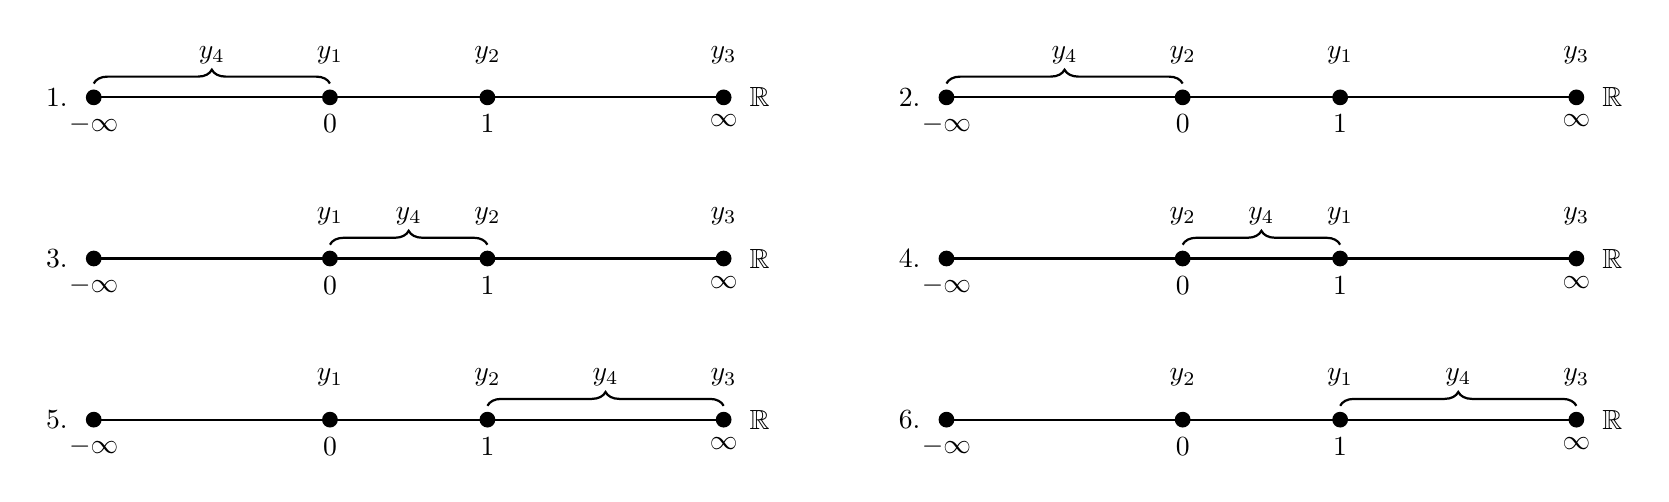
\begin{tikzpicture}[
    brc/.style args = {#1/#2}{decorate,decoration={brace,amplitude=5pt,raise=#1,#2},thick},
  ]


  \matrix (A) [column sep=40,row sep=20] {
    \pic (A1) {realline={y_1}{y_2}{y_3}};
    \draw[brc=5/] (A1-1) -- node[above=3mm] {$y_4$} (A1-4);

     & \pic (A2) {realline={y_2}{y_1}{y_3}};
    \draw[brc=5/] (A2-1) -- node[above=3mm] {$y_4$} (A2-4);
    \\

    \pic (A3) {realline={y_1}{y_2}{y_3}};
    \draw[brc=5/] (A3-4) -- node[above=3mm] {$y_4$} (A3-6);

     & \pic (A4) {realline={y_2}{y_1}{y_3}};
    \draw[brc=5/] (A4-4) -- node[above=3mm] {$y_4$} (A4-6);
    \\

    \pic (A5) {realline={y_1}{y_2}{y_3}};
    \draw[brc=5/] (A5-6) -- node[above=3mm] {$y_4$} (A5-9);

     & \pic (A6) {realline={y_2}{y_1}{y_3}};
    \draw[brc=5/] (A6-6) -- node[above=3mm] {$y_4$} (A6-9);
    \\
  };
\end{tikzpicture}
\end{document}